% If enabled, this produces a notes-free version for handing out
%\def\HANDOUT{}
% If enabled in tandem with \HANDOUT, doesn't reformat the slides to fit on a
% single page
%\def\EMAILEDCOPY{}

% The paper: https://arxiv.org/pdf/2508.07177

\documentclass[
    aspectratio=169,
    \ifdefined\HANDOUT
    handout
    \else
    \fi
]{beamer}
\usetheme{AnnArbor}
\usecolortheme{illini}
\setbeamertemplate{note page}[]
\ifdefined\HANDOUT
\ifdefined\EMAILEDCOPY
\else
\usepackage{pgfpages}
\pgfpagesuselayout{resize to}[letterpaper,border shrink=2mm, landscape]
\fi
\else
%\setbeameroption{show notes}
%\setbeameroption{show notes on second screen=bottom}
\fi
\setbeamertemplate{caption}[numbered]

% Automatically add Section Title Slids
\AtBeginSection[]{
  \begin{frame}
  \vfill
  \centering
  \begin{beamercolorbox}[sep=8pt,center,shadow=true,rounded=true]{title}
    \usebeamerfont{title}\insertsectionhead\par%
  \end{beamercolorbox}
  \vfill
  \end{frame}
}

%TODO Font should be adjusted (bigger)
\usepackage[]{amsfonts}
\newcommand{\overbar}[1]{\mkern 1.5mu\overline{\mkern-1.5mu#1\mkern-1.5mu}\mkern 1.5mu}
\usepackage{amsmath}
\usepackage{amssymb}
\usepackage{mathtools}
\usepackage{listings}
\usepackage{algorithm}
\usepackage{algpseudocode}
\usepackage{ulem}
\usepackage{censor}

%\usepackage{biblatex}
%\renewcommand*{\bibfont}{\small}

\DeclareMathOperator*{\argmax}{arg\,max}
\DeclareMathOperator*{\argmin}{arg\,min}

\graphicspath{img}

\title[PHYS 595]{``An Analogy of Frequency Droop Control for Grid-forming Sources''}
\subtitle{A PHYS 595 Journal Club Presentation}
\author[ES]{Eric Silk}
\institute[ECE@UIUC]{Electrical and Computer Engineering\linebreak University of Illinois at Urbana-Champaign}
\date{April 24th, 2026}
\logo{
\includegraphics[height=1cm]{img/small_logo.png}}
\begin{document}
\definecolor{UIUCOrange}{RGB}{255,95,5}
\definecolor{UIUCBlue}{RGB}{19,41,75}
\definecolor{UIUCBlueSubhead}{RGB}{5,86,165}
\definecolor{UIUCBlueKnockoutheader}{RGB}{32,64,151}
\definecolor{UIUCGray1}{RGB}{232,233,234}
\definecolor{UIUCGray2}{RGB}{166,168,171}
\definecolor{UIUCGray3}{RGB}{94,102,105}

\begin{frame}
    \titlepage
    \tiny
    Compiled: \today
\end{frame}


%\begin{frame}
%    \tableofcontents
%\end{frame}

\section{Background}
\begin{frame}
    \frametitle{Motivation}
    \begin{itemize}
        \item Principally pedagogical
        \item Mechanical analogy for electrical system
        \item Useful for education and intuition when designing power systems
        \item Not research, \textit{per se}
    \end{itemize}

\end{frame}
\begin{frame}
    \frametitle{Power Generation}
    \begin{columns}
        \begin{column}{0.5\textwidth}
            \begin{itemize}
                \item Power is alternating current (AC)
                \item Historically highly centralized
                \item Uses \textit{synchronous machines}
                \item System frequency is proportional to power balance
                \item Strong coupling between grid dynamics and generator behavior
            \end{itemize}
        \end{column}
        \begin{column}{0.5\textwidth}
            \begin{figure}[h]
                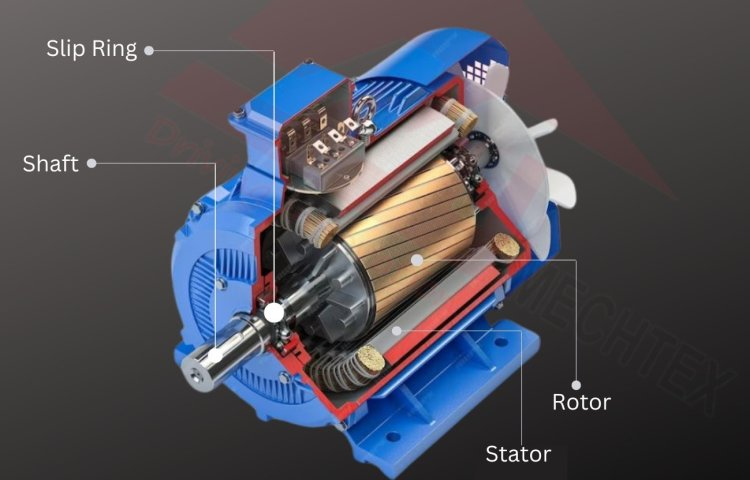
\includegraphics[width=0.9\textwidth]{img/synch_machine.jpg}
                \caption{A cutaway render of a synchronous machine\cite{synch_machine}}
            \end{figure}
        \end{column}
    \end{columns}
\end{frame}

\begin{frame}
    \frametitle{Primary Control}
    \begin{columns}
        \begin{column}{0.5\textwidth}
            \begin{itemize}
                \item Inverse relationship between frequency and speed
                \item Droop control
                \item Prevents frequency collapse
                \item Enables power sharing between generators
                \item ``Grid forming'' (GFM) resources
            \end{itemize}
            \vspace{10pt}
            \begin{equation}
                f = f_{nom}-m_p\left(P-P_{ref}\right)
            \end{equation}
            \begin{equation}
                m_p\coloneqq \frac{\Delta f}{S_{rated}}
            \end{equation}
        \end{column}
        \begin{column}{0.5\textwidth}
            \begin{figure}[h]
                \vspace{-10pt}
                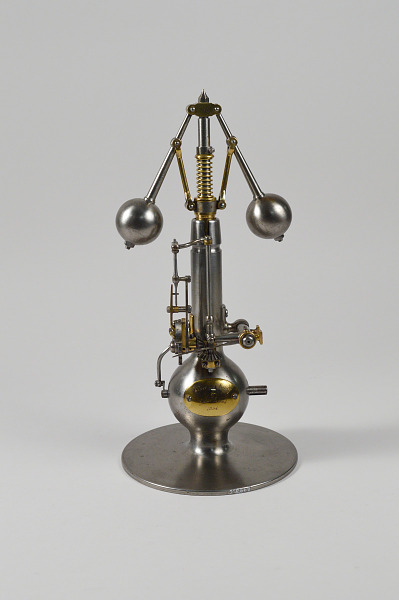
\includegraphics[height=0.6\textheight]{img/guvnah.jpg}
                \caption{An early form of primary control: a steam engine governor\cite{guvnah}}
            \end{figure}
        \end{column}
    \end{columns}
\end{frame}

\begin{frame}
    \frametitle{Inverter Based Resources}
    \begin{columns}
        \begin{column}{0.5\textwidth}
            \begin{itemize}
                \item Some resources produce \textit{direct} current (DC)
                \item This must be converted to AC via \textit{inverters}
                \item Similar to digital-to-analog converters (DACs)
                \item Weakly coupled to grid dynamics
                \item Historically ``grid following'' (GFL), converting to GFM
            \end{itemize}
        \end{column}
        \begin{column}{0.5\textwidth}
            \begin{figure}[h]
                \vspace{-10pt}
                \includegraphics[height=0.6\textheight]{img/solar_panels.png}
                \caption{An example of an inverter-based resource (the solar panels)}
            \end{figure}
        \end{column}
    \end{columns}
\end{frame}


\section{Key Results}
\subsection{The Analogy}
\begin{frame}
    \begin{block}{Question}
        \begin{center}
            How can we reframe these abstract/hard to visualize electrical quantities?
        \end{center}
    \end{block}
    \begin{block}{Answer}\pause
        \begin{center}
            Convert them by mathematical analogy to some \textit{physical} system
        \end{center}
    \end{block}
\end{frame}
\begin{frame}
    \frametitle{Basic Visual}
    \begin{figure}[h]
        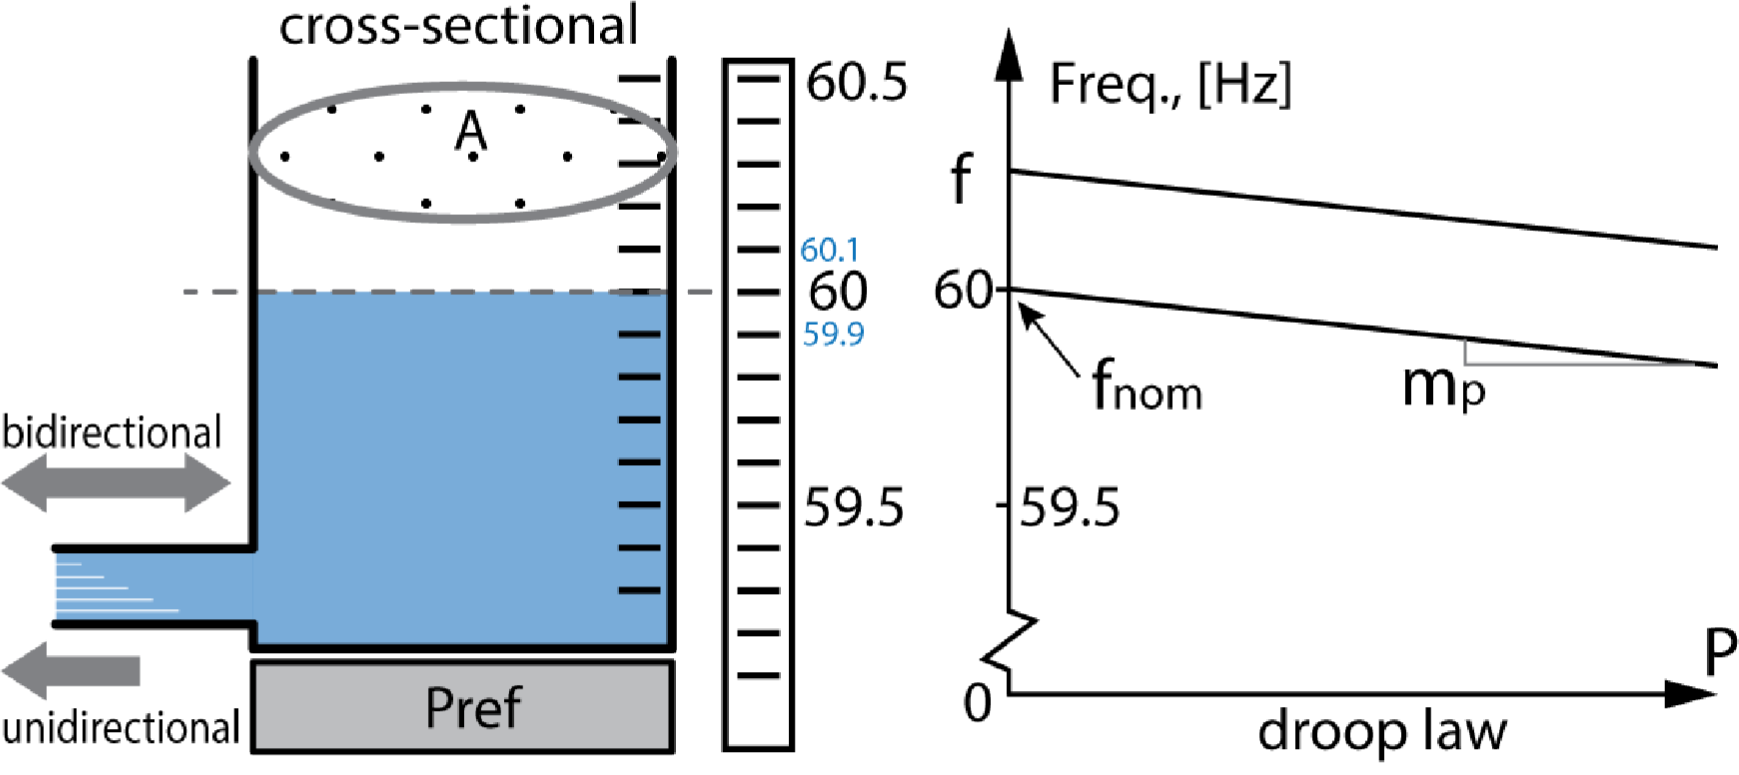
\includegraphics[width=0.85\textwidth]{img/physical_analogy.png}
        \caption{The basic analogy, with the associated droop curve\cite{main_paper}}
    \end{figure}
\end{frame}

\begin{frame}
    \frametitle{Comparable Values}
    \begin{table}[]
        \begin{tabular}{l|ll}
            Symbol    & Communicating Vessels                     & GFM sources        \\ \hline
            $f$       & \multicolumn{1}{l|}{Water Level}          & Actual Frequency   \\
            $f_{nom}$ & \multicolumn{1}{l|}{Base Reference Level} & Nominal Frequency  \\
            $A$       & \multicolumn{1}{l|}{Cross-sectional Area} & Reciprocal of m\_p \\
            $m_p$     & \multicolumn{1}{l|}{Reciprocal of A}      & Droop slope        \\
            $P$       & \multicolumn{1}{l|}{Outflow Water Amount} & Real Power         \\
            $P_{ref}$ & \multicolumn{1}{l|}{Block Elevation}      & Power Setpoint     \\
            $L$       & \multicolumn{1}{l|}{Pipes}                & Electrical Cables
        \end{tabular}
    \end{table}
\end{frame}

\begin{frame}
    \frametitle{Nonlinear Controls}
    \begin{figure}[h]
        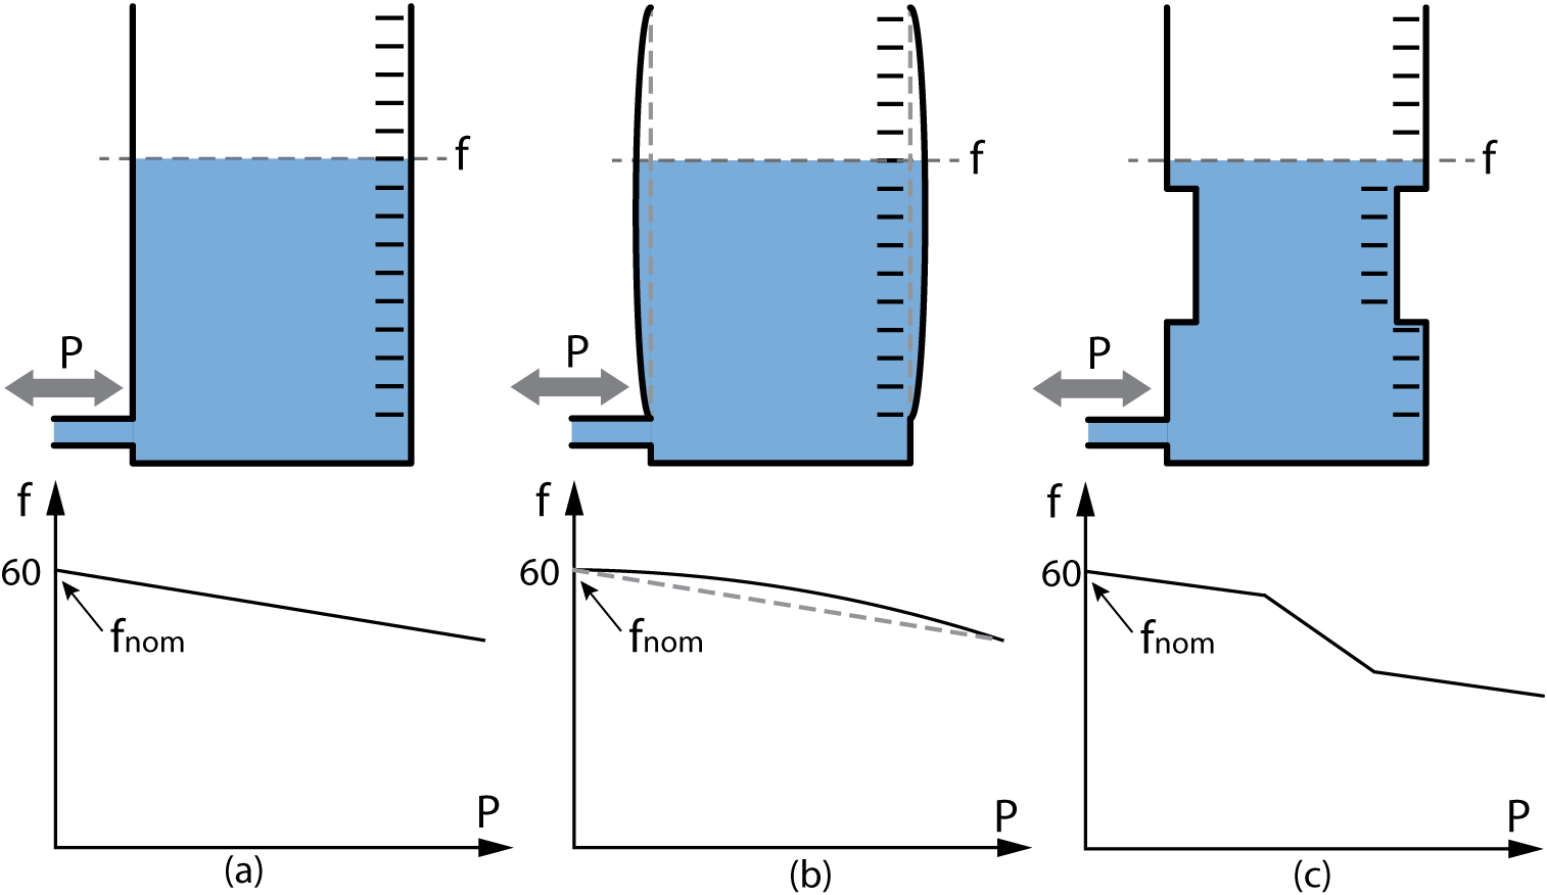
\includegraphics[height=0.7\textheight]{img/nonlinear.png}
        \caption{Various droop shapes: Linear (a), convex curved (b), and piecewise linear (c)\cite{main_paper}}
    \end{figure}
\end{frame}

\subsection{Applications/Demonstration}
\begin{frame}
    \frametitle{Power Setpoints and Grid Connection}
    \begin{figure}[h]
        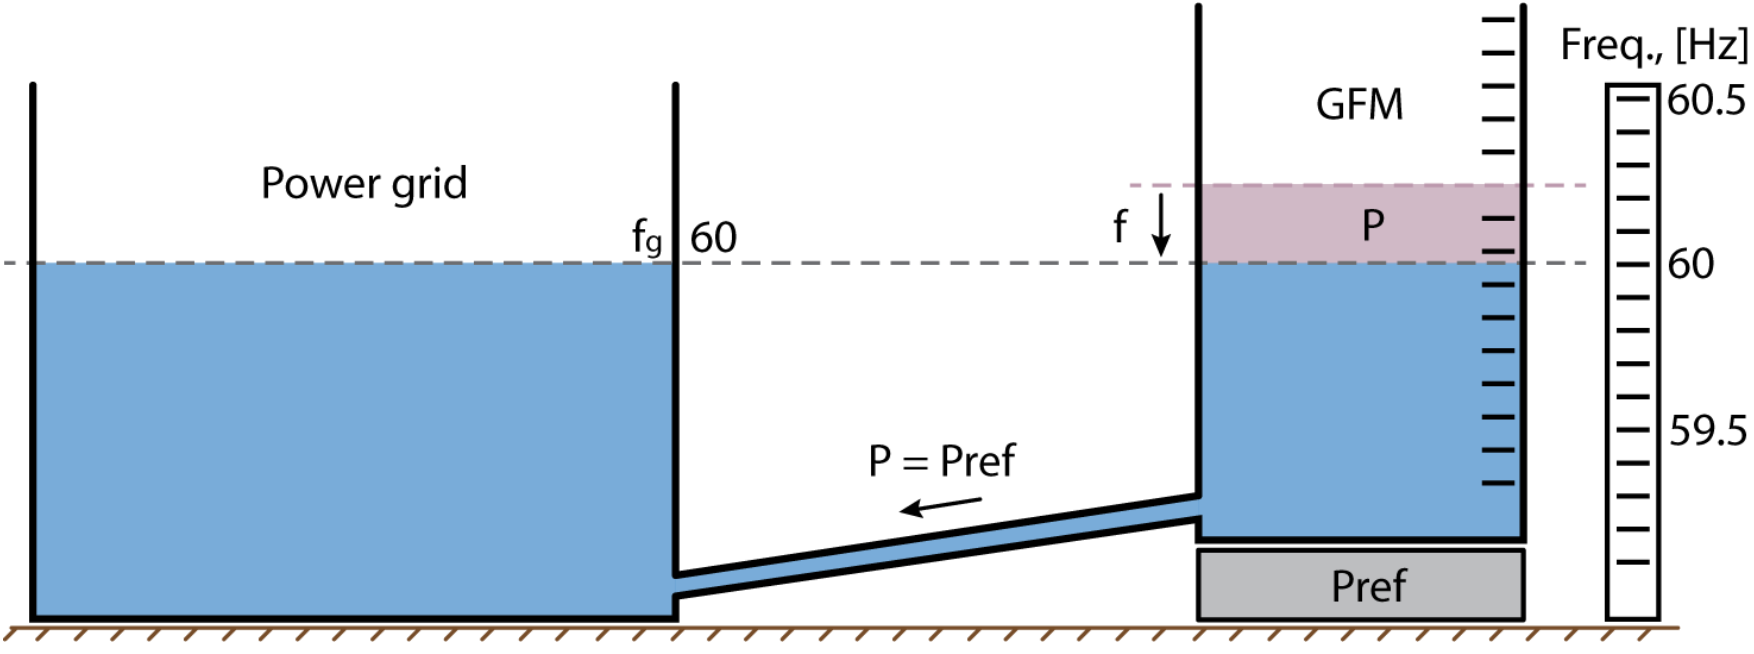
\includegraphics[height=0.65\textheight]{img/grid_connected.png}
        \caption{Various droop shapes: Linear (a), convex curved (b), and piecewise linear (c)\cite{main_paper}}
    \end{figure}
\end{frame}
\begin{frame}
    \frametitle{Interconnected GFM Resources}
    \begin{figure}[h]
        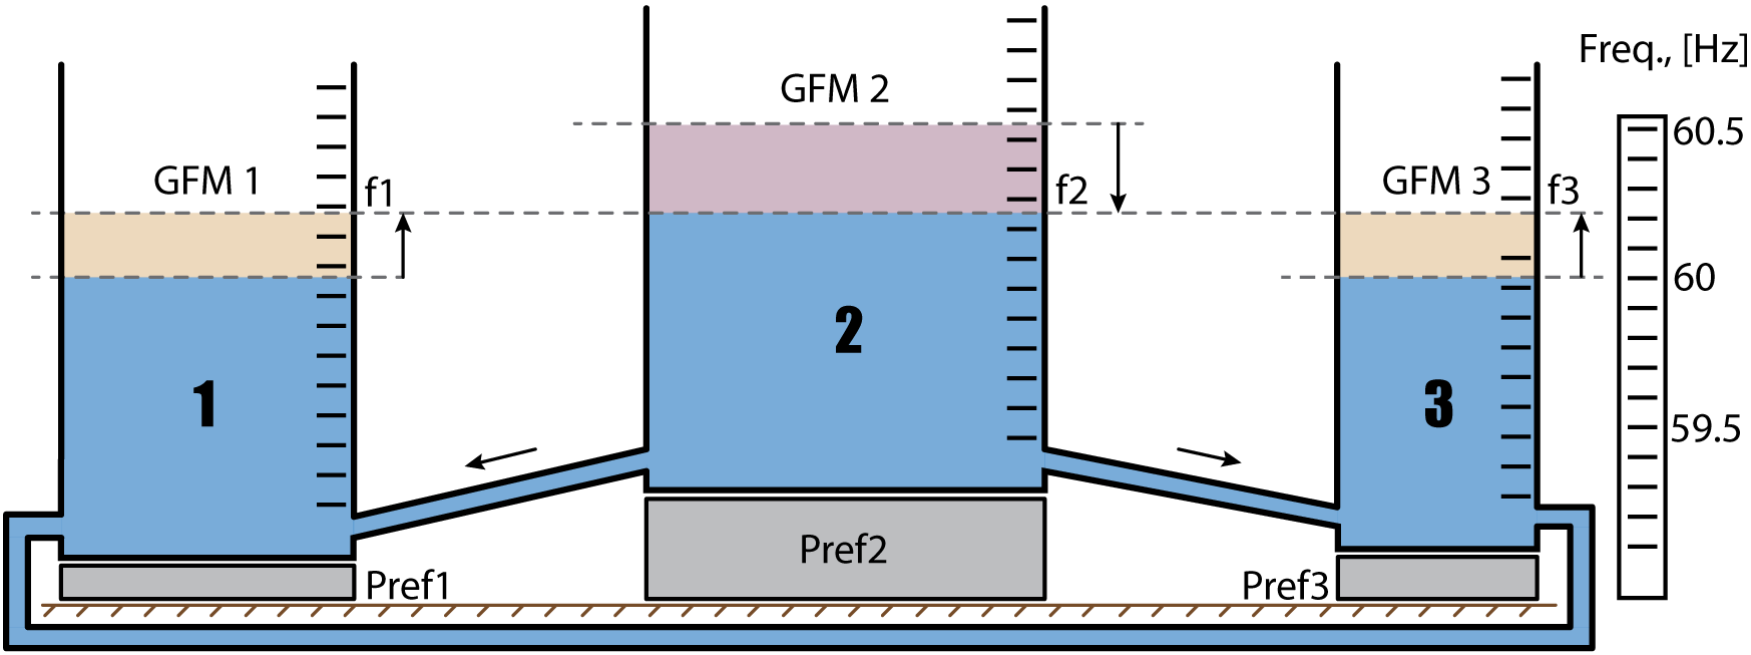
\includegraphics[height=0.65\textheight]{img/interconnected.png}
        \caption{Frequency regulation/power sharing among interconnected resources\cite{main_paper}}
    \end{figure}
\end{frame}
\begin{frame}
    \frametitle{Microgrid}
    \begin{figure}[h]
        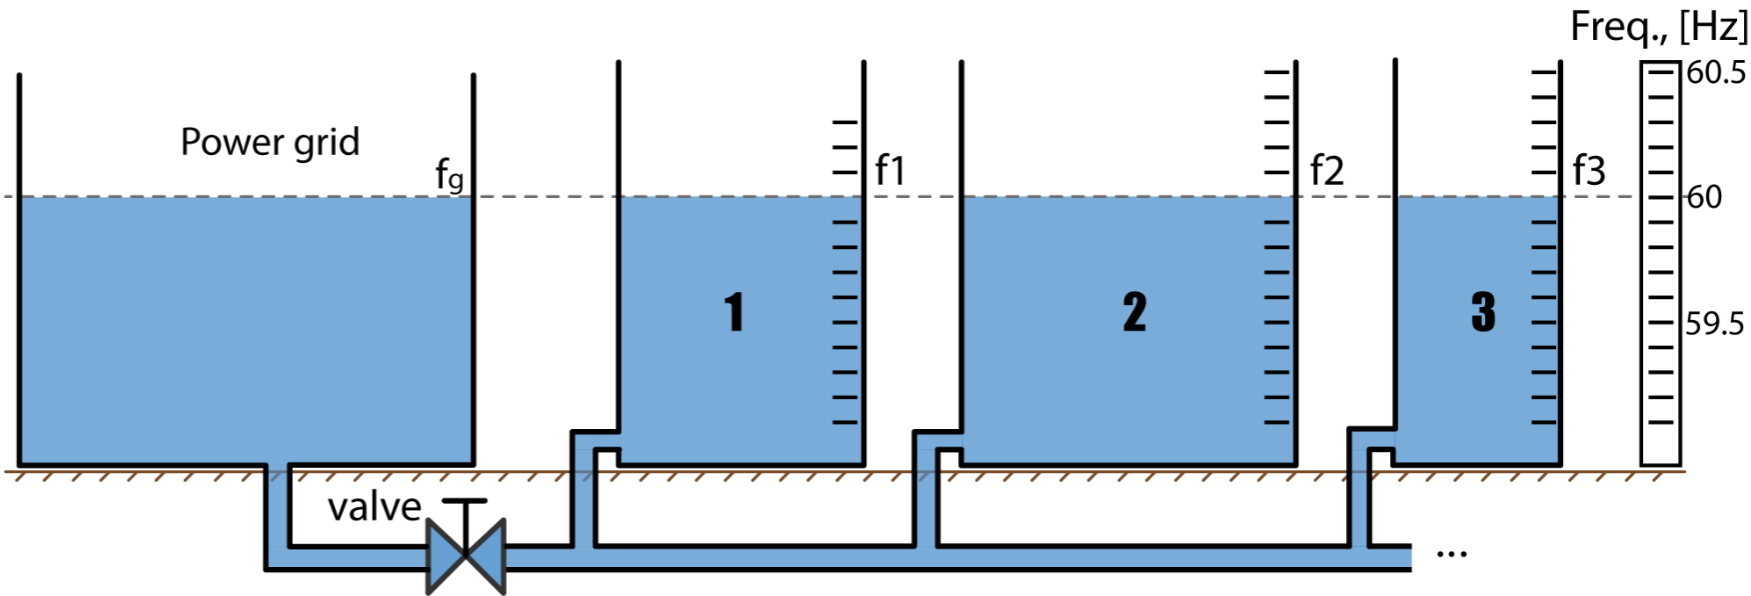
\includegraphics[height=0.65\textheight]{img/microgrid.png}
        \caption{An example microgrid, showing the ability to island via a valve\cite{main_paper}}
    \end{figure}
\end{frame}

\begin{frame}
    \frametitle{Numerical Results}
    \begin{columns}
        \begin{column}{0.5\textwidth}
            \begin{itemize}
                \item Several numerical simulations included
                \item Ultimately, nothing surprising here
            \end{itemize}
        \end{column}
        \begin{column}{0.5\textwidth}
            \begin{figure}[h]
                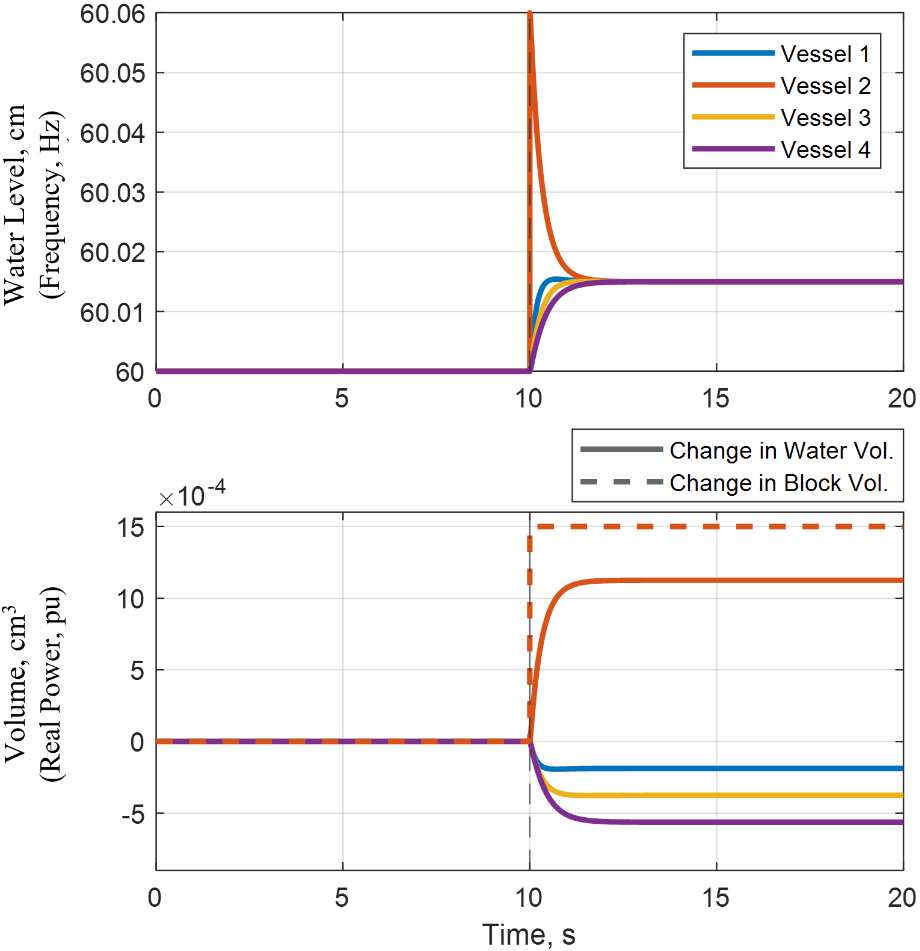
\includegraphics[height=0.5\textheight]{img/numerical.png}
                \caption{Simulation of changing the power/block setpoint\cite{synch_machine}}
            \end{figure}
        \end{column}
    \end{columns}
\end{frame}

\section{Critical Response}
\begin{frame}
    \frametitle{Importance}
    \begin{columns}
        \begin{column}{0.5\textwidth}
            \begin{block}{Negatives}
                \begin{itemize}
                    \item Water-tank analogy already exists for droop control in synchronous machines
                    \item IBR droop control is designed to be identical
                    \item Analogy for GFM's is thus trivial
                \end{itemize}
            \end{block}
        \end{column}
        \begin{column}{0.5\textwidth}
            \begin{block}{Positives}
                \begin{itemize}
                    \item The nonlinear/piecewise linear examples are perhaps not obvious
                    \item Could be a useful for new researchers in this space
                    \item Old results, but with new language and examples
                \end{itemize}
            \end{block}
        \end{column}
    \end{columns}
\end{frame}

\begin{frame}
    \frametitle{Broad Interest and Accessibility}
    \begin{columns}
        \begin{column}{0.5\textwidth}
            \begin{block}{Positives}
                \begin{itemize}
                    \item Extremely approachable analogy
                    \item Good visuals and examples
                    \item Modifications to base example laid out logically
                \end{itemize}
            \end{block}
        \end{column}
        \begin{column}{0.5\textwidth}
            \begin{block}{Negatives}
                \begin{itemize}
                    \item Insufficent background for non-power audience
                    \item Insufficient motivation for alternative controls
                \end{itemize}
            \end{block}
        \end{column}
    \end{columns}
\end{frame}

\section{Conclusion}
\begin{frame}
    \frametitle{Concluding Remarks}
\end{frame}
\begin{frame}
    \frametitle{Bibliography}
    \bibliographystyle{amsalpha}
    {
        \tiny
        \bibliography{qual_presentation.bib}
    }
\end{frame}

\end{document}